\documentclass{beamer}
\usepackage[utf8]{inputenc}
\usepackage[italian]{babel}
\usepackage{graphicx}
\usepackage{booktabs}
\usepackage{tikz}
\usepackage{adjustbox}

\usetheme{Amurmaple}
\setbeamertemplate{navigation symbols}{}%remove navigation symbols
\title[Travelling Salesman Problem]{Esplorazione delle Soluzioni al TSP: Algoritmi Esatti e Red-Black ACS}
\author{Mouhieddine Sabir}
\institute[UniPD]{Università degli Studi di Padova}
\date{Settembre 2024}


\begin{document}

\frame{\titlepage}

\begin{frame}
    \frametitle{Sommario}
    \tableofcontents
\end{frame}

\section{Introduzione}
\tiny
\begin{frame}{Introduzione al TSP e Formulazione Matematica}
    \begin{block}{Definizione del Problema del Commesso Viaggiatore (TSP)}
        \begin{itemize}
            \item Trovare il percorso più breve che visiti ogni città una volta e torni all'inizio
            \item Applicazioni: logistica, ingegneria, genomica, astronomia
        \end{itemize}
    \end{block}

    \begin{block}{Formulazione Matematica}
        \begin{itemize}
            \item Modello: minimizzare $\sum_{i=1}^{n} \sum_{j=1, j \neq i}^{n} c_{ij} x_{ij}$ su grafo $G = (V, E)$
            \item Vincoli: ogni città visitata una sola volta
            \item Varianti: STSP, ATSP, TSPTW
        \end{itemize}
    \end{block}

    \begin{block}{Algoritmi Esatti}
        \begin{itemize}
            \item Brute Force: $O(n!)$, per problemi piccoli
            \item Bellman-Held-Karp: $O(n^2 \cdot 2^n)$, programmazione dinamica
            \item Concorde TSP Solver: branch-and-cut, per istanze grandi
        \end{itemize}
    \end{block}
\end{frame}

\section{Algoritmi Euristici e Metaeuristici}
\begin{frame}{Algoritmi Euristici}
    \textbf{Nearest Neighbor (NNS)}
    \begin{itemize}
        \item Seleziona la città più vicina non ancora visitata.
        \item Soluzione veloce, ma non ottimale.
    \end{itemize}
    \textbf{2-opt e 3-opt}
    \begin{itemize}
        \item Tecniche di ottimizzazione locale: scambiano segmenti del tour per ridurre la lunghezza.
        \item 2-opt: scambio di due lati.
        \item 3-opt: scambio di tre lati.
    \end{itemize}


    \begin{table}
        \centering
        \caption{Risultati NN vs NN+2Opt}
        \begin{tabular}{lllrrrr}
            \toprule
               & Istanza  & algorithm & Tempo (ms) & Lunghezza Tour & Lunghezza ottima & Gap   \\
            \midrule
            0  & berlin52 & NN        & 14         & 8980.92        & 7542.00          & 19.08 \\
            1  & berlin52 & NN2Opt    & 124        & 8060.65        & 7542.00          & 6.88  \\
            2  & d198     & NN        & 183        & 18620.07       & 15780.00         & 18.00 \\
            3  & d198     & NN2Opt    & 4443       & 16165.31       & 15780.00         & 2.44  \\
            4  & eil76    & NN        & 17         & 711.99         & 538.00           & 32.34 \\
            5  & eil76    & NN2Opt    & 313        & 599.05         & 538.00           & 11.35 \\
            6  & fl1577   & NN        & 9547       & 27940.91       & 22249.00         & 25.58 \\
            7  & fl1577   & NN2Opt    & 200151     & 24214.30       & 22249.00         & 8.83  \\
            8  & lin105   & NN        & 43         & 20362.76       & 14379.00         & 41.61 \\
            9  & lin105   & NN2Opt    & 2959       & 16199.70       & 14379.00         & 12.66 \\
            10 & lin318   & NN        & 466        & 54033.58       & 42029.00         & 28.56 \\
            11 & lin318   & NN2Opt    & 9562       & 46408.41       & 42029.00         & 10.42 \\
            12 & rl5915   & NN        & 236473     & 707498.63      & 565530.00        & 25.10 \\
            13 & rl5915   & NN2Opt    & 6327036    & 620822.08      & 565530.00        & 9.78  \\
            14 & u574     & NN        & 1295       & 46881.87       & 36905.00         & 27.03 \\
            15 & u574     & NN2Opt    & 26923      & 39896.00       & 36905.00         & 8.10  \\
            \bottomrule
        \end{tabular}
    \end{table}
\end{frame}
\section{Algoritmi Metaeuristici}
\begin{frame}{Simulated Annealing (SA)}
    \textbf{Principio di Base}
    \begin{itemize}
        \item Ispirato al processo fisico della ricottura dei metalli, dove una sostanza viene riscaldata e poi raffreddata lentamente per raggiungere uno stato a bassa energia.
        \item Simulated Annealing (SA) applica questo concetto all'ottimizzazione, cercando di evitare ottimi locali accettando temporaneamente soluzioni peggiori con una certa probabilità.
    \end{itemize}

    \textbf{Funzionamento}
    \begin{itemize}
        \item Si parte con una soluzione iniziale e una temperatura iniziale elevata.
        \item Viene esplorato il vicinato della soluzione corrente, generando una nuova soluzione candidata.
        \item Se la soluzione candidata è migliore, viene accettata. Se è peggiore, può essere accettata con una probabilità che decresce con la temperatura.
        \item La temperatura viene gradualmente ridotta durante il processo (cooling schedule).
    \end{itemize}
    \begin{table}[H]
        \centering
        \caption{Risultati SA vs SA2Opt}
        \begin{tabular}{lllrrrr}
            \toprule
               & Istanza  & algorithm & Tempo (ms) & Lunghezza Tour & Lunghezza ottima & Gap   \\
            \midrule
            0  & berlin52 & SA        & 28982      & 7544.37        & 7542.00          & 0.03  \\
            1  & berlin52 & SA2Opt    & 49481      & 7544.37        & 7542.00          & 0.03  \\
            2  & d198     & SA2Opt    & 93813      & 16118.48       & 15780.00         & 2.14  \\
            3  & d198     & SA        & 102362     & 16318.76       & 15780.00         & 3.41  \\
            4  & eil76    & SA        & 39587      & 572.81         & 538.00           & 6.47  \\
            5  & eil76    & SA2Opt    & 45721      & 569.29         & 538.00           & 5.82  \\
            6  & fl1577   & SA        & 1514830    & 27584.16       & 22249.00         & 23.98 \\
            7  & fl1577   & SA2Opt    & 2391057    & 23489.49       & 22249.00         & 5.58  \\
            8  & lin105   & SA        & 52928      & 14993.92       & 14379.00         & 4.28  \\
            9  & lin105   & SA2Opt    & 54366      & 14882.69       & 14379.00         & 3.50  \\
            10 & lin318   & SA2Opt    & 392433     & 45444.25       & 42029.00         & 8.13  \\
            11 & lin318   & SA        & 506369     & 47651.44       & 42029.00         & 13.38 \\
            12 & rl5915   & SA2Opt    & 18690779   & 615257.00      & 565530.00        & 8.79  \\
            13 & rl5915   & SA        & 22563370   & 680777.61      & 565530.00        & 20.38 \\
            14 & u574     & SA2Opt    & 369840     & 39443.68       & 36905.00         & 6.88  \\
            15 & u574     & SA        & 398181     & 43936.09       & 36905.00         & 19.05 \\
            \bottomrule
        \end{tabular}
    \end{table}
\end{frame}

\begin{frame}{Algoritmi Genetici (GA)}
    \textbf{Principio di Base}
    \begin{itemize}
        \item Ispirato dalla teoria dell'evoluzione naturale di Darwin. Le soluzioni del problema sono trattate come individui in una popolazione che evolve nel tempo.
        \item Utilizza concetti di selezione, crossover (incrocio) e mutazione per generare nuove soluzioni.
    \end{itemize}

    \textbf{Funzionamento}
    \begin{itemize}
        \item Si parte con una popolazione iniziale di soluzioni (cromosomi), ciascuna delle quali rappresenta una possibile soluzione al problema.
        \item Le soluzioni vengono valutate secondo una funzione di fitness, che misura la qualità della soluzione.
        \item Le migliori soluzioni vengono selezionate per generare nuove soluzioni attraverso crossover, combinando le caratteristiche di due "genitori" per creare un "figlio".
        \item Viene introdotta la mutazione per mantenere la diversità nella popolazione, evitando di convergere troppo presto su un ottimo locale.
    \end{itemize}
    \begin{table}[H]
        \centering

        \caption{Risultati GA vs GA+2Opt}
        \begin{tabular}{lllrrrr}
            \toprule
               & Istanza  & algorithm & Tempo (ms) & Lunghezza Tour & Lunghezza ottima & Gap     \\
            \midrule
            0  & berlin52 & GA2Opt    & 26104      & 7918.09        & 7542.00          & 4.99    \\
            1  & berlin52 & GA        & 29932      & 11009.32       & 7542.00          & 45.97   \\
            2  & d198     & GA2Opt    & 108498     & 16548.42       & 15780.00         & 4.87    \\
            3  & d198     & GA        & 137106     & 66868.76       & 15780.00         & 323.76  \\
            4  & eil76    & GA2Opt    & 44547      & 570.63         & 538.00           & 6.06    \\
            5  & eil76    & GA        & 45556      & 977.18         & 538.00           & 81.63   \\
            6  & fl1577   & GA        & 2264528    & 1116417.45     & 22249.00         & 4917.83 \\
            7  & fl1577   & GA2Opt    & 4033113    & 24024.81       & 22249.00         & 7.98    \\
            8  & lin105   & GA2Opt    & 109871     & 14573.34       & 14379.00         & 1.35    \\
            9  & lin105   & GA        & 164073     & 44653.50       & 14379.00         & 210.55  \\
            10 & lin318   & GA2Opt    & 320190     & 45165.59       & 42029.00         & 7.46    \\
            11 & lin318   & GA        & 429314     & 363904.18      & 42029.00         & 765.84  \\
            12 & rl5915   & GA        & 20712540   & 38904633.04    & 565530.00        & 6779.32 \\
            13 & rl5915   & GA2Opt    & 33367821   & 648205.16      & 565530.00        & 14.62   \\
            14 & u574     & GA        & 471427     & 457563.15      & 36905.00         & 1139.84 \\
            15 & u574     & GA2Opt    & 1260895    & 40516.22       & 36905.00         & 9.79    \\
            \bottomrule
        \end{tabular}
    \end{table}
\end{frame}

\section{Ant Colony System (ACS)}
\begin{frame}{Ant Colony System (ACS)}
    \textbf{Principio di Base}
    \begin{itemize}
        \item Ispirato al comportamento delle colonie di formiche nel cercare il cibo. Le formiche depositano una sostanza chimica (feromone) lungo il percorso mentre cercano il cibo, rafforzando i percorsi più brevi.
        \item Nel contesto del TSP, le formiche artificiali esplorano il grafo delle città e aggiornano i percorsi (archi) in base alla qualità della soluzione trovata.
    \end{itemize}

    \textbf{Funzionamento}
    \begin{itemize}
        \item Ogni formica inizia da una città casuale e costruisce iterativamente un tour visitando città non ancora visitate.
        \item La probabilità che una formica scelga una determinata città è basata su due fattori: la quantità di feromone su quell’arco e l'inverso della distanza (euristica).
        \item Dopo che tutte le formiche hanno completato il loro tour, si aggiorna il feromone sugli archi. I percorsi migliori vengono rinforzati con più feromone.
        \item Viene utilizzato un meccanismo di evaporazione per evitare che i feromoni si accumulino troppo e bloccano l'esplorazione di nuove soluzioni.
    \end{itemize}

    \textbf{Regole di Aggiornamento}
    \begin{itemize}
        \item \textbf{Aggiornamento locale}: Durante la costruzione del tour, una formica aggiorna localmente il livello di feromone dell’arco che attraversa.
        \item \textbf{Aggiornamento globale}: Solo la formica con il miglior tour globale aggiorna il livello di feromone sull’intero percorso.
    \end{itemize}
    \begin{table}[H]
        \centering
        \caption{Risultati ACS vs ACS+2Opt}
        \begin{tabular}{lllrrrr}
            \toprule
               & Istanza  & algorithm & Tempo (ms) & Lunghezza Tour & Lunghezza ottima & Gap   \\
            \midrule
            0  & berlin52 & ACS       & 18411      & 7606.66        & 7542.00          & 0.86  \\
            1  & berlin52 & ACS2Opt   & 20289      & 7598.44        & 7542.00          & 0.75  \\
            2  & d198     & ACS       & 94445      & 16584.44       & 15780.00         & 5.10  \\
            3  & d198     & ACS2Opt   & 101484     & 16079.65       & 15780.00         & 1.90  \\
            4  & eil76    & ACS2Opt   & 27703      & 558.76         & 538.00           & 3.86  \\
            5  & eil76    & ACS       & 33136      & 554.04         & 538.00           & 2.98  \\
            6  & fl1577   & ACS       & 2880286    & 25939.85       & 22249.00         & 16.59 \\
            7  & fl1577   & ACS2Opt   & 3852624    & 22914.07       & 22249.00         & 2.99  \\
            8  & lin105   & ACS2Opt   & 80683      & 14605.88       & 14379.00         & 1.58  \\
            9  & lin105   & ACS       & 123877     & 14981.78       & 14379.00         & 4.19  \\
            10 & lin318   & ACS2Opt   & 202670     & 43556.33       & 42029.00         & 3.63  \\
            11 & lin318   & ACS       & 338493     & 46646.52       & 42029.00         & 10.99 \\
            12 & rl5915   & ACS2Opt   & 34991642   & 612104.64      & 565530.00        & 8.24  \\
            13 & rl5915   & ACS       & 35872198   & 706188.19      & 565530.00        & 24.87 \\
            14 & u574     & ACS       & 452117     & 42512.54       & 36905.00         & 15.19 \\
            15 & u574     & ACS2Opt   & 490206     & 39051.51       & 36905.00         & 5.82  \\
            \bottomrule
        \end{tabular}
    \end{table}


\end{frame}


\section{Red-Black Ant Colony System (RB-ACS)}
\begin{frame}{Red-Black Ant Colony System (RB-ACS)}
    \textbf{Motivazioni e Introduzione}
    \begin{itemize}
        \item Variante migliorata dell'Ant Colony System (ACS) sviluppata per migliorare l’efficienza e la precisione.
        \item Introduce due gruppi di formiche (Rosse e Nere), ognuno dei quali lavora in parallelo su percorsi separati.
    \end{itemize}

    \textbf{Funzionamento}
    \begin{itemize}
        \item \textbf{Inizializzazione}: Le formiche di entrambi i gruppi iniziano con una distribuzione uniforme dei feromoni.
        \item \textbf{Esecuzione in parallelo}: Le formiche rosse e nere operano indipendentemente, ma aggiornano i feromoni globali alla fine di ogni iterazione.
        \item \textbf{Aggiornamento dei Feromoni}: I percorsi globalmente migliori vengono potenziati utilizzando il contributo combinato di entrambi i gruppi.
    \end{itemize}

    \textbf{Vantaggi}
    \begin{itemize}
        \item Migliora l'esplorazione dello spazio delle soluzioni grazie alla diversificazione tra i gruppi.
        \item Mantiene un bilanciamento tra esplorazione e sfruttamento delle soluzioni ottimali.
    \end{itemize}

    \begin{table}[H]
        \centering
        \caption{Risultati RB-ACS vs RB-ACS+2Opt}
        \begin{tabular}{lllrrrr}
            \toprule
               & Istanza  & algorithm & Tempo (ms) & Lunghezza Tour & Lunghezza ottima & Gap   \\
            \midrule
            0  & berlin52 & RBACS     & 34002      & 7681.45        & 7542.00          & 1.85  \\
            1  & berlin52 & RBACS2Opt & 34159      & 7544.37        & 7542.00          & 0.03  \\
            2  & d198     & RBACS     & 136998     & 17097.74       & 15780.00         & 8.35  \\
            3  & d198     & RBACS2Opt & 283417     & 16076.46       & 15780.00         & 1.88  \\
            4  & eil76    & RBACS     & 40567      & 562.41         & 538.00           & 4.54  \\
            5  & eil76    & RBACS2Opt & 40672      & 557.14         & 538.00           & 3.56  \\
            6  & fl1577   & RBACS     & 4210934    & 26788.92       & 22249.00         & 20.41 \\
            7  & fl1577   & RBACS2Opt & 6887456    & 23236.46       & 22249.00         & 4.44  \\
            8  & lin105   & RBACS     & 77720      & 14785.44       & 14379.00         & 2.83  \\
            9  & lin105   & RBACS2Opt & 262217     & 14489.08       & 14379.00         & 0.77  \\
            10 & lin318   & RBACS     & 469358     & 46823.70       & 42029.00         & 11.41 \\
            11 & lin318   & RBACS2Opt & 603140     & 43421.71       & 42029.00         & 3.31  \\
            12 & rl5915   & RBACS     & 21861319   & 716108.43      & 565530.00        & 26.63 \\
            13 & rl5915   & RBACS2Opt & 28403435   & 608329.94      & 565530.00        & 7.57  \\
            14 & u574     & RBACS     & 826684     & 43702.95       & 36905.00         & 18.42 \\
            15 & u574     & RBACS2Opt & 899785     & 39219.59       & 36905.00         & 6.27  \\
            \bottomrule
        \end{tabular}
    \end{table}
\end{frame}

\begin{frame}{Confronto degli Approcci al TSP}
    \small
    \begin{columns}[T,totalwidth=\textwidth]
        \begin{column}{0.5\textwidth}
            \textbf{Esatti}
            \begin{itemize}
                \item[+] Soluzione ottimale
                \item[-] Alta complessità
            \end{itemize}

            \textbf{Euristici}
            \begin{itemize}
                \item[+] Veloci
                \item[-] Non ottimali
            \end{itemize}

            \textbf{Simulated Annealing}
            \begin{itemize}
                \item[+] Evita ottimi locali
                \item[-] Convergenza lenta
            \end{itemize}
        \end{column}

        \begin{column}{0.5\textwidth}
            \textbf{Genetici}
            \begin{itemize}
                \item[+] Adattabili
                \item[-] Costo computazionale
            \end{itemize}

            \textbf{Ant Colony System}
            \begin{itemize}
                \item[+] Efficace su problemi complessi
                \item[-] Molti parametri
            \end{itemize}

            \textbf{Red-Black ACS}
            \begin{itemize}
                \item[+] Migliore esplorazione dello spazio
                \item[-] Maggiore complessità computazionale
            \end{itemize}
        \end{column}
    \end{columns}
\end{frame}

\section{Risultati Sperimentali}
\begin{frame}{Heatmap}
    \adjustbox{width=\paperwidth,height=\paperheight,keepaspectratio}{%
        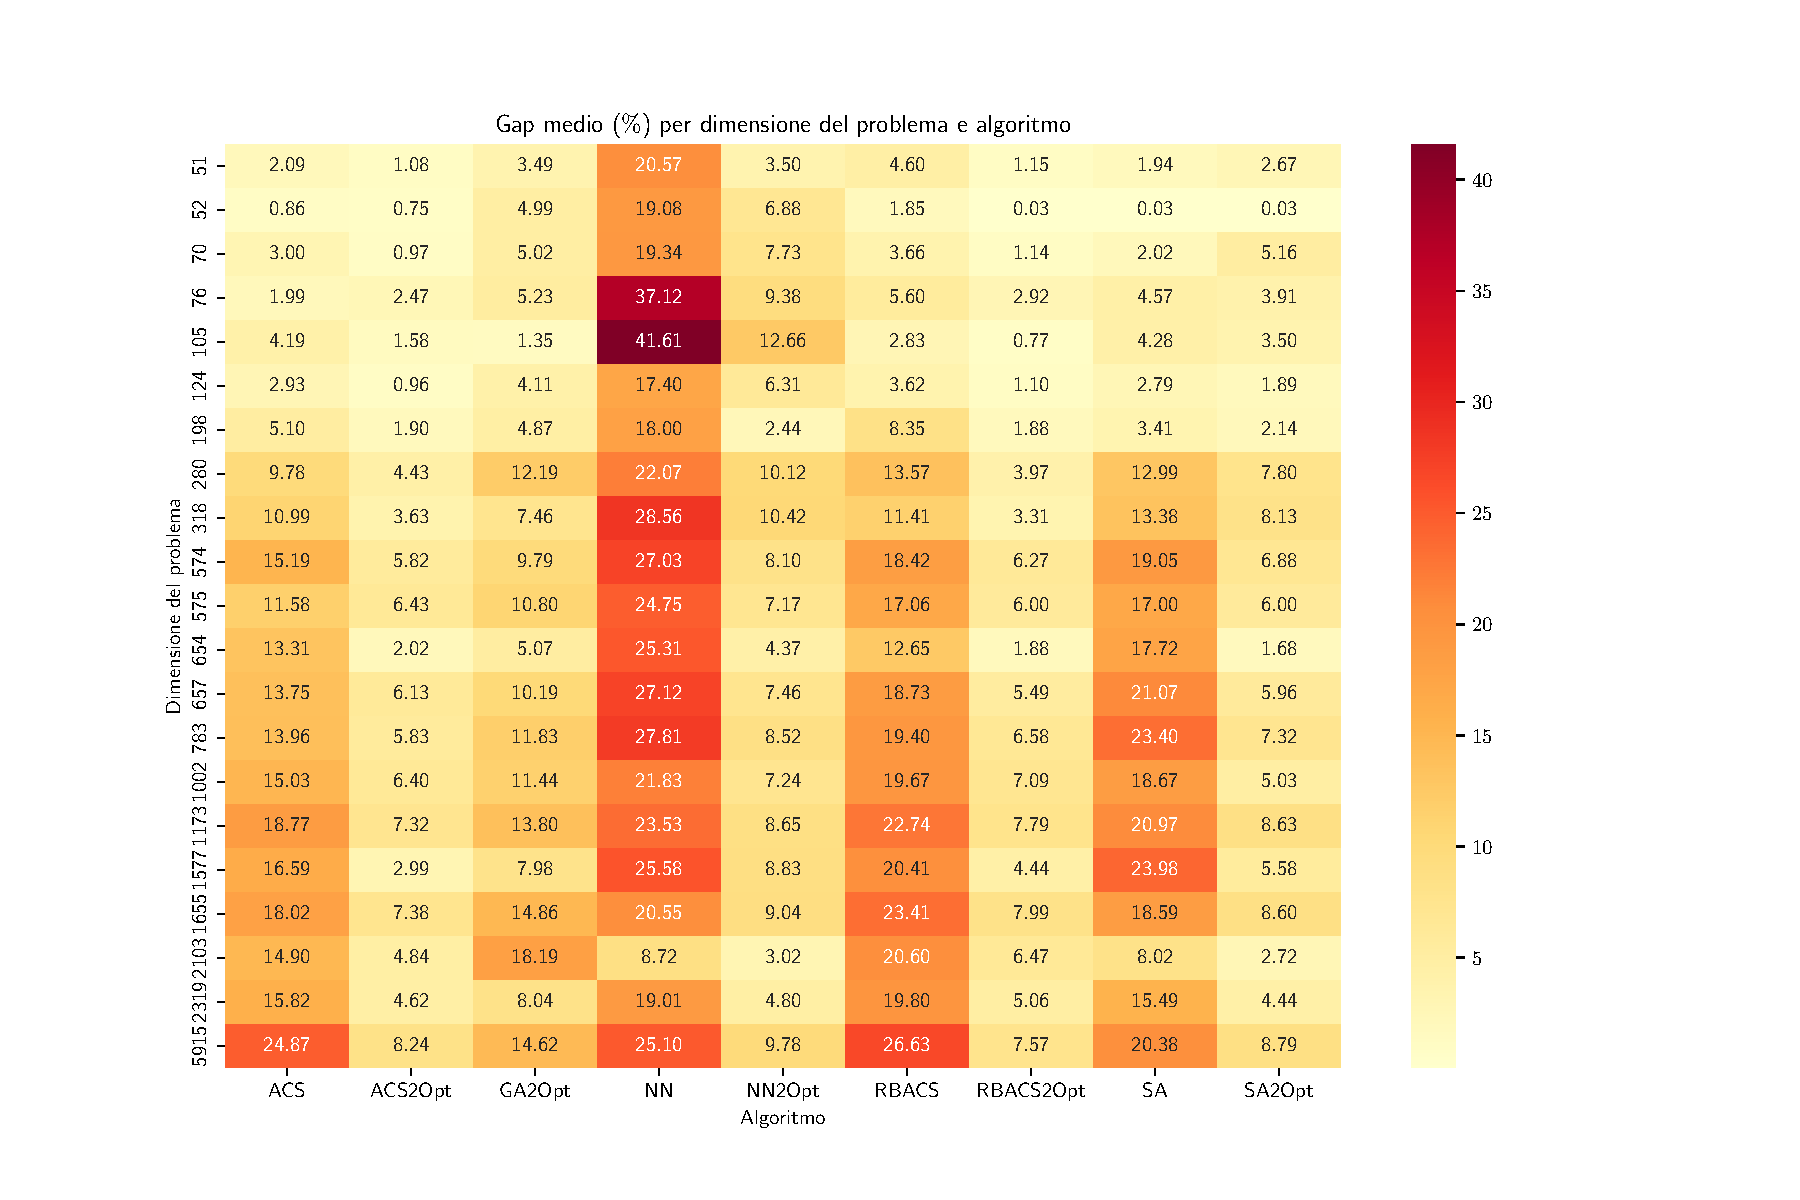
\includegraphics{analysis/heatmap_full.pdf}%
    }
\end{frame}

\begin{frame}{Confronto degli Algoritmi}
    \adjustbox{width=0.90\paperwidth,height=\paperheight,keepaspectratio}{%
        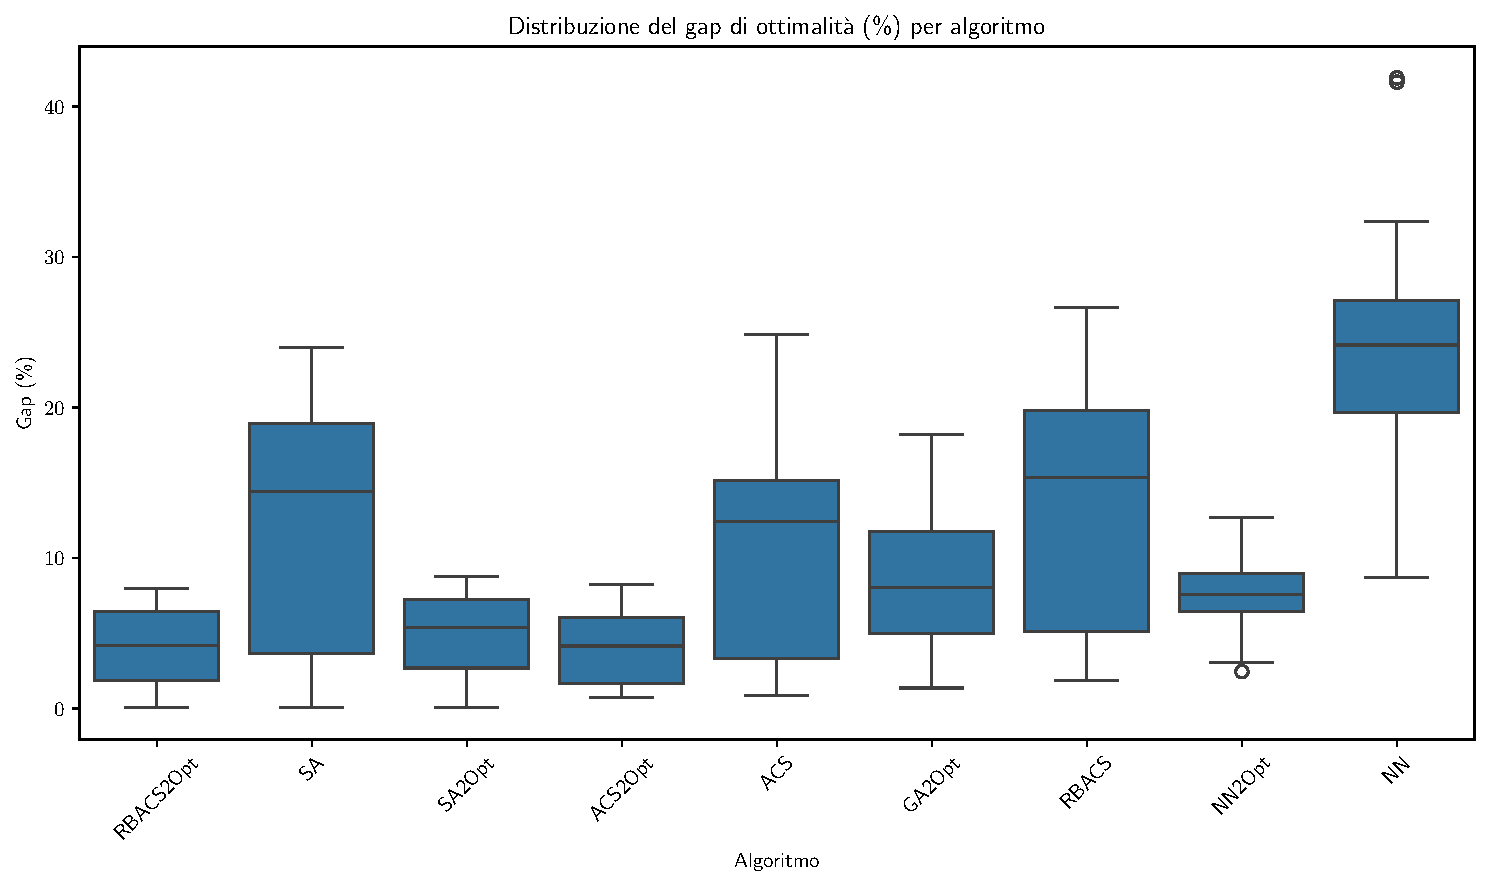
\includegraphics{analysis/alg_comparison.pdf}%
    }
\end{frame}

\section{Conclusioni}
\begin{frame}{Conclusioni}
    \begin{itemize}
        \item Il Red-Black Ant Colony System (RB-ACS) ha dimostrato di essere un approccio promettente per la risoluzione del TSP e altri problemi di ottimizzazione combinatoria.
        \item Sebbene più complesso computazionalmente rispetto ad ACS, l'uso di due gruppi di formiche (Rosse e Nere) con parametri e strategie di aggiornamento differenziati consente una migliore esplorazione dello spazio delle soluzioni.
        \item Questo approccio ha portato a miglioramenti significativi nelle prestazioni, in particolare su istanze di grandi dimensioni.
        \item In alcuni casi, il RB-ACS ha superato gli approcci tradizionali, dimostrando il potenziale del suo design per affrontare le sfide computazionali dei problemi NP-hard.
        \item Studi futuri potrebbero estendere il RB-ACS ad altre varianti del TSP e ad altri problemi di ottimizzazione per verificare ulteriormente la sua efficacia.
    \end{itemize}
\end{frame}


\end{document}
